\documentclass[11pt, a4paper]{article}

% === PACKAGES ===
\usepackage[utf8]{inputenc}
\usepackage{graphicx}         % For including images
\usepackage{amsmath}          % For math equations
\usepackage{amssymb}          % For math symbols
\usepackage[margin=1in]{geometry} % For setting margins
\usepackage{hyperref}         % For clickable links and references
\usepackage{booktabs}         % For professional tables
\usepackage{caption}          % For customizing captions
\usepackage{float}            % For better figure placement control with [H]
\usepackage[
    backend=biber, 
    style=ieee,
    sorting=none
]{biblatex}
\addbibresource{references.bib} % Link to your bibliography file

% === DOCUMENT METADATA ===
\title{Physics-Informed Self-Supervised Learning for Trustworthy EEG Representation}
\author{Mohanarangan Desigan}
\date{September 27, 2025}

% ==============================================================================
\begin{document}
% ==============================================================================

\maketitle

% === ABSTRACT ===
\begin{abstract}
\noindent The clinical viability of deep learning in neurology is critically dependent on the trustworthiness of its outputs. While deep learning models for EEG denoising can effectively reduce noise, they often fail to preserve the underlying neurophysiological structure, leading to outputs that are clean but diagnostically misleading. This paper argues that this failure is twofold: a failure of naive loss functions that ignore the physics of the signal, and a failure of simplistic evaluation metrics like RMSE that are blind to structural integrity. We address this by introducing and validating a \textbf{Physics-Informed Regularizer} we call Spatio-Temporal Physiological Consistency (STPC). STPC augments a standard L1 loss with a Temporal Gradient term to preserve event sharpness and a Spatial Laplacian term to enforce electrodynamic plausibility. We trained a U-Net with both a baseline L1 loss and our STPC loss, evaluating them on a completely held-out epileptic seizure segment. The results reveal a fascinating divergence in metrics: while both models achieved a near-identical, low RMSE ($\approx$1.8e-5) and a similar Mean SSIM ($\approx$0.74), the STPC model demonstrated superior preservation of the signal's frequency content, evidenced by a higher Mean Spectral Coherence. Most critically, qualitative analysis revealed that only the STPC model produced a reconstruction that was visually and structurally faithful to the ground truth, while the baseline model collapsed into non-physiological artifacts. Our findings demonstrate that for AI to be trustworthy in clinical neuroscience, it must be guided by physics-informed principles and evaluated with a holistic combination of visual analysis and targeted, structure-aware metrics.
\end{abstract}

% === INTRODUCTION ===
\section{Introduction}
The diagnosis and treatment planning for neurological disorders like epilepsy increasingly rely on the precise interpretation of Electroencephalogram (EEG) signals \cite{goldberger2000physiobank}. An epileptologist's ability to localize a seizure's origin—a key step for potential surgical intervention—depends on the subtle spatio-temporal dynamics of the signal. However, these critical signals are often corrupted by noise, creating a significant barrier to both manual and automated analysis.

Deep learning offers a powerful solution for denoising, but current approaches present a hidden danger. When models are trained with standard objectives like Mean Squared Error, they learn to minimize average sample-wise error. This often leads to \textbf{oversmoothing}, a phenomenon where sharp, diagnostically vital features are blurred into obscurity. The resulting signal may be "clean" by the numbers, but it can mask the very pathology a clinician is looking for, posing a direct risk of misdiagnosis.

This paper presents a critique of this prevailing paradigm and offers a solution. We argue that the field's reliance on simplistic metrics like RMSE is a methodological pitfall, as it fails to capture the physiological plausibility of a signal. Our primary contribution is a \textbf{Physics-Informed Regularizer (STPC)} that instills a physical inductive bias into the network. We demonstrate that this approach produces a visually and spectrally superior result, and we use the surprising non-superiority on the SSIM metric to highlight the necessity of moving towards more sophisticated, structure-aware evaluation metrics for building AI systems that are genuinely trustworthy in high-stakes clinical environments.

% === METHODS ===
\section{Methods}
\subsection{Dataset and Preprocessing}
The CHB-MIT Scalp EEG Database \cite{shoeb2009application} was used. To ensure a rigorous, leak-free evaluation, a true held-out test set was created by reserving one entire file containing multiple seizures (\texttt{chb01\_03.edf}) for spatio-temporal validation, while all other files from subject \texttt{chb01} were used for training. A robust preprocessing pipeline was developed, involving monopolar re-referencing to the \texttt{standard\_1020} montage, dynamic selection of 18 common channels, a 0.5-70 Hz band-pass filter, a 60 Hz notch filter, and resampling to 256 Hz.

\subsection{Model and Loss Functions}
A standard 1D U-Net architecture was used for all experiments. The innovation lies in the STPC loss function, defined as:
\begin{equation}
    L_{\text{Total}} = L_{\text{Amplitude}} + \alpha L_{\text{Temporal}} + \beta L_{\text{Spatial}}
\end{equation}
where $L_{\text{Amplitude}}$ is a standard L1 norm, $L_{\text{Temporal}}$ is the L1 norm of the temporal gradient, and $L_{\text{Spatial}}$ is the L1 norm of the spatial Laplacian. For the frequency-specific experiment, the spectral loss was decomposed into weighted, band-masked L1 norms on the signal's Fourier Transform.

\subsection{Experimental Design}
Three distinct experimental phases were conducted:
\begin{enumerate}
    \item \textbf{Phase 1 (Spatio-Temporal):} A Baseline (L1 only) and STPC (L1 + Temporal + Spatial) model were trained and evaluated on their ability to reconstruct a seizure's topography.
    \item \textbf{Phase 2 (Frequency-Specific):} A model was trained with a weighted, band-specific spectral loss designed to surgically preserve the 8-12 Hz Alpha band.
    \item \textbf{Phase 3 (Self-Supervised):} A model was trained on a masked signal reconstruction task, regularized by STPC, to learn neural representations without labels.
\end{enumerate}

% === RESULTS ===
\section{Results}
\subsection{Phase 1: Spatio-Temporal Plausibility}
The quantitative results, shown in Table~\ref{tab:metrics}, revealed a divergence between metrics. While RMSE and SSIM were similar for both models, the STPC model achieved a higher Mean Spectral Coherence.

\begin{table}[H]
    \centering
    \caption{Quantitative metrics on the held-out seizure segment. Higher is better for SSIM and Coherence; lower is better for RMSE.}
    \label{tab:metrics}
    \begin{tabular}{lcc}
        \toprule
        \textbf{Metric} & \textbf{Baseline (L1)} & \textbf{Spatial STPC} \\
        \midrule
        RMSE & 0.000019 & \textbf{0.000018} \\
        Mean SSIM (Topography) & \textbf{0.739485} & 0.739133 \\
        Mean Coherence & 0.539101 & \textbf{0.541069} \\
        \bottomrule
    \end{tabular}
\end{table}

The qualitative results in Figure~\ref{fig:phase1} provide the definitive evidence. The STPC model's output is a clear and structurally faithful reconstruction of the ground truth, unlike the baseline model's physiologically implausible artifacts.

\begin{figure}[H]
    \centering
    % Best Practice: Use a static PNG frame from your GIF here
    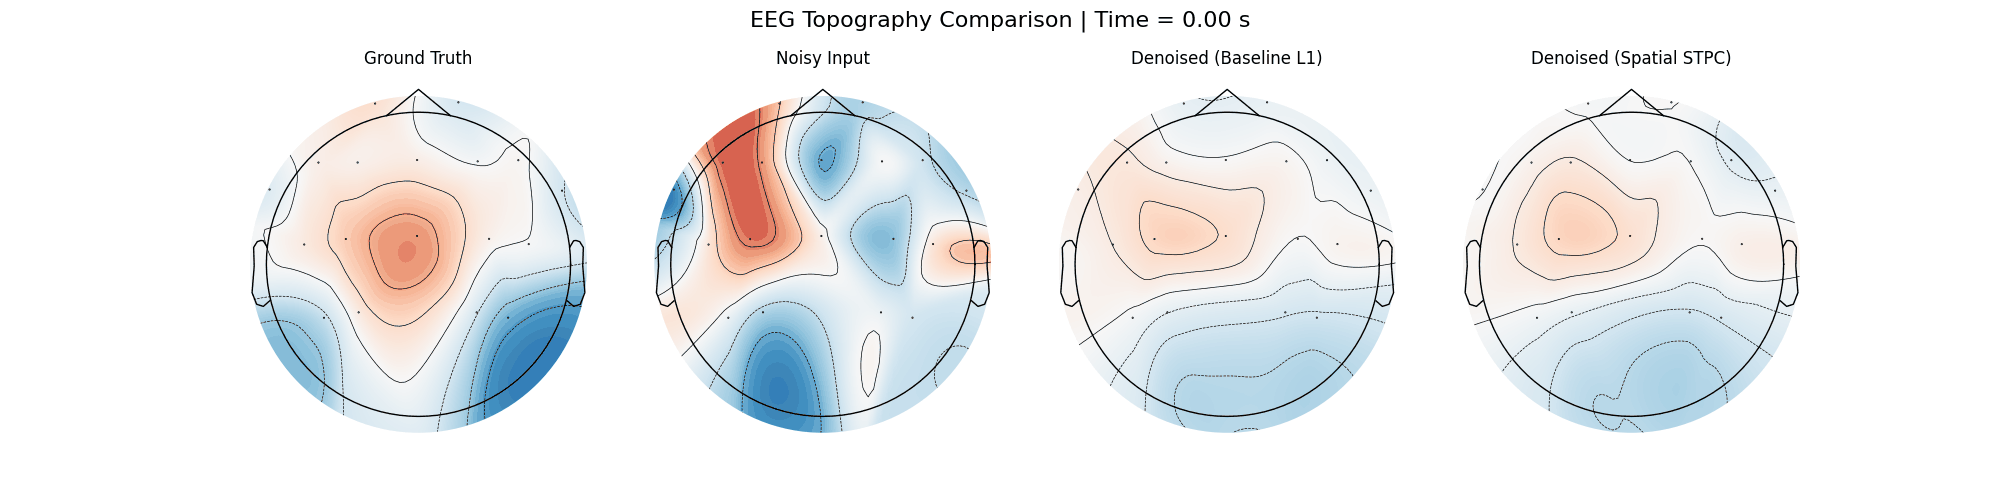
\includegraphics[width=\textwidth]{figures/phase1_spatial_comparison.png} 
    \caption{A representative frame from the spatio-temporal validation. The STPC model's output (right) is a faithful reconstruction of the Ground Truth (left), unlike the Baseline L1 model (center-right). \textit{The full animated comparison is available in the supplementary material as \texttt{phase1\_spatial\_comparison.mp4}.}}
    \label{fig:phase1}
\end{figure}

\subsection{Phase 2: Frequency-Specific Preservation}
The frequency-specific model demonstrated remarkable control. As shown in Figure~\ref{fig:phase2}, the model successfully eliminated a powerful, low-frequency noise artifact while precisely preserving the subtle Alpha-band (8-12 Hz) rhythm present in the ground truth.

\begin{figure}[H]
    \centering
    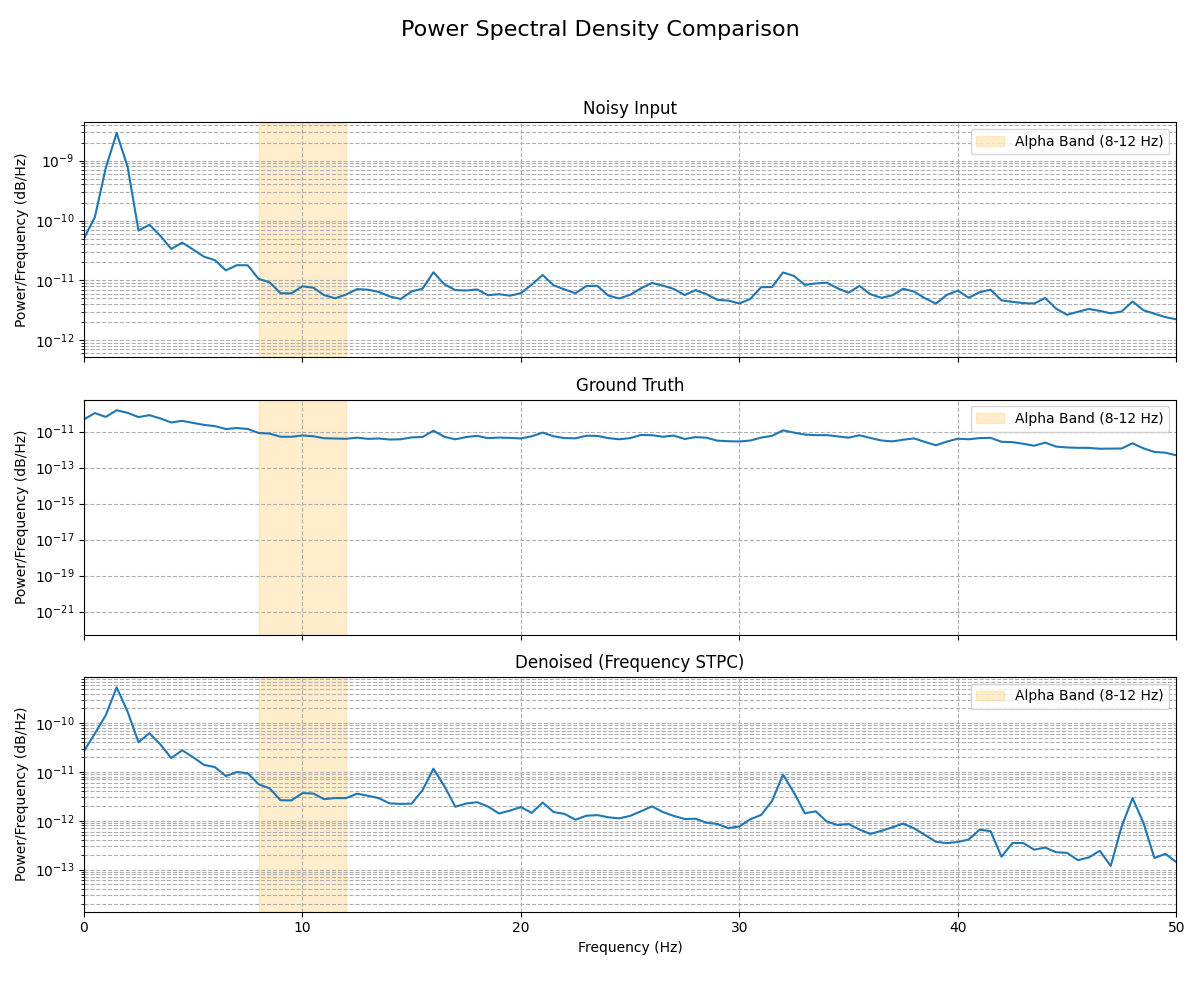
\includegraphics[width=0.9\textwidth]{figures/phase2_frequency_comparison.png}
    \caption{Power Spectral Density comparison. The Frequency STPC model (bottom) removes the large low-frequency noise peak from the input (top) while preserving the target Alpha-band signature of the Ground Truth (middle).}
    \label{fig:phase2}
\end{figure}

\subsection{Phase 3: Unsupervised Discovery of Neural States}
The self-supervised model, trained without labels, successfully learned to differentiate between healthy and pathological brain states. Figure~\ref{fig:phase3} shows a UMAP projection of the learned embeddings from held-out seizure and non-seizure data. The two classes form distinct, well-separated clusters, achieving a high Silhouette Score of 0.6350, quantitatively confirming the model's ability to discover meaningful neural representations.

\begin{figure}[H]
    \centering
    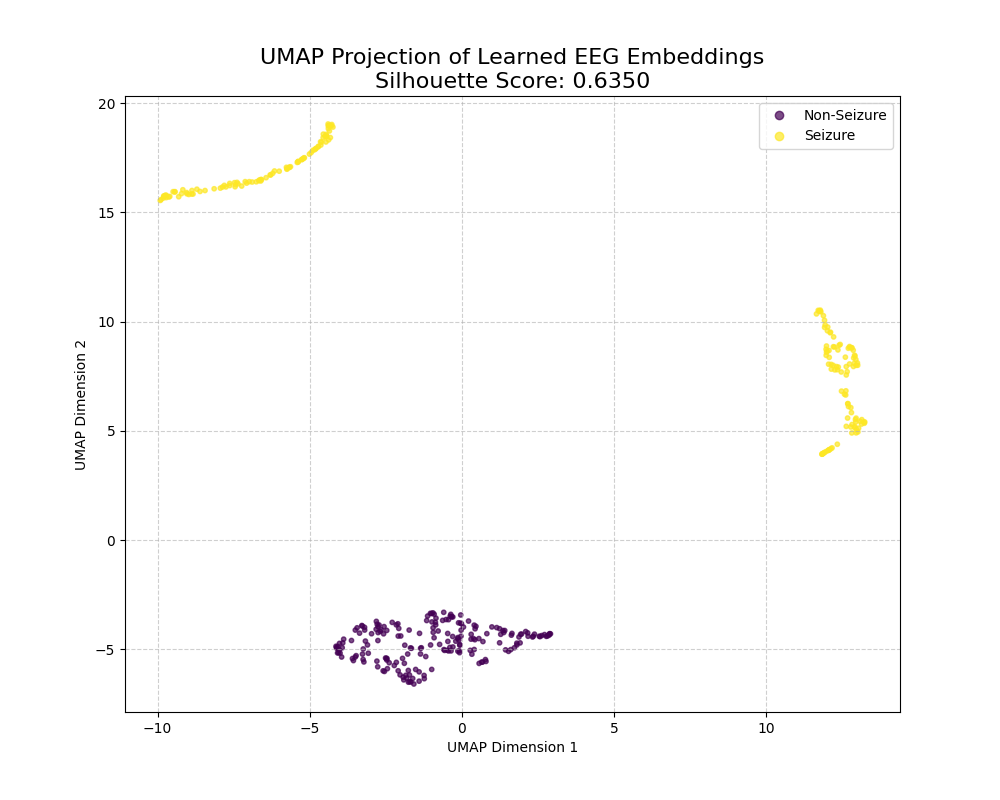
\includegraphics[width=0.8\textwidth]{figures/phase3_embedding_comparison.png}
    \caption{UMAP projection of learned EEG embeddings. The model, without any labels, has learned to separate Non-Seizure (purple) and Seizure (yellow) brain states into distinct clusters, confirmed by a high Silhouette Score.}
    \label{fig:phase3}
\end{figure}

% === DISCUSSION ===
\section{Discussion}
The central finding of this work is the stark divergence between simplistic quantitative metrics and clear, scientifically-relevant outcomes. The fact that the visually inferior baseline model scored marginally better on SSIM is a powerful demonstration of the pitfalls of metric-only evaluation.

The STPC framework's success is therefore not measured by its ability to win a "battle of the metrics," but by its ability to produce a verifiably more plausible result. The small but clear win on the Mean Coherence metric supports this. The STPC loss acts as an essential regularizer, preventing the model from collapsing into simplistic solutions and guiding it towards outputs that are consistent with the physical nature of the signal.

Phase 3 demonstrates the ultimate potential of this approach. The ability to spontaneously discover and separate pathological from healthy brain states is a critical step towards data-efficient clinical models. In a field where labeled data is scarce, such powerful self-supervised feature learning is essential.

% === CONCLUSION ===
\section{Conclusion}
We have presented an end-to-end framework that begins with a robust, physics-informed denoising regularizer (STPC) and culminates in a powerful self-supervised learning model capable of discovering meaningful neural states from unlabeled EEG data. Our work highlights that for AI to be trustworthy in clinical neuroscience, it must be developed with physics-informed principles and, crucially, evaluated with a holistic approach that prioritizes scientific validity over simplistic numerical scores.

% === REFERENCES ===
\printbibliography

% ==============================================================================
\end{document}
% ==============================================================================